\documentclass{llncs}
\usepackage[utf8]{inputenc}
\usepackage{llncsdoc}
\usepackage{graphicx}
\usepackage{hyperref}
\usepackage{listings}
\usepackage{color}

\newcommand{\inlinecode}{\texttt}

\begin{document}

\title{Fault Tolerance for PCJ}

\author{Michał Szynkiewicz}
\institute{Faculty of Mathematics and Computer Science Nicolaus Copernicus University, Toruń, Poland}

\date{2015}
\maketitle

\begin{abstract}

Nowadays, distributed computations are often run on large amounts of nodes for a significant amount of time.
Having a 24 hour long computation on 1000 nodes means almost 3 years of computations.
As calculated in \cite{RX10}, with 6 month mean time between failures, it gives less than 1\% chance of success.

PCJ library is a high-performance parallel computing library for Java implementing PGAS model.

This paper describes changes introduced in PCJ to provide basic fault tolerance and fault tolerance strategies that are planned to be implemented in future.

\end{abstract}

\section{Introduction}
Before the changes described in this paper, any network or hardware failure resulted in hanging of a PCJ-based program.

The changes introduce \emph{Ignore failure} fault tolerance policy.
This is a minimum-overhead, no-checkpoint strategy.

For programs that do not require results from all nodes to finish, like Monte Carlo randomized algorithms, the strategy is enough to finish calculations properly.
For other programs, the strategy provides a useful base on which the programmer may build a dedicated solution (e.g. replaying failed nodes work on other node).


\section{PCJ library}
PCJ library is a Java implementation of PGAS model.
It is fast, lightweight and it ships as a single jar.

The smallest unit of computation in PCJ is called a \emph{thread}. Each \emph{thread} has its own local address space and shared address space.
The owner \emph{thread} accesses local and global address spaces variables as usual Java fields.

Multiple \emph{threads} may be run on one physical machine, within a single Java Virtual Machine (JVM).
A \emph{thread} or group of \emph{threads} run on a single JVM are called a \emph{node}.

PCJ distinguishes one node, namely \emph{node 0}. This is the start node for all computations.

Following is a description of PCJ features. For more details please see \cite{pcj-manual}.
\subsection{Synchronization}\label{sync}
Threads synchronization in PCJ is realized by \inlinecode{barrier}.
Barrier can be made either across all threads or two threads.
In first case each task has to call \inlinecode{barrier} method.
Barrier is managed by \emph{node 0} and realized in two steps.
First, each node on which all threads have called \inlinecode{barrier} informs \emph{node 0} that it has reached \inlinecode{barrier} and starts waiting.
When \emph{node 0} gathers barrier confirmations from all nodes, it releases the barrier by broadcasting a specific message to all nodes.
Broadcasting is realized in an efficient way described later.
\subsection{Shared memory}
Fields that should be put into shared address space have to be annotated in \inlinecode{@Shared} annotation.
Aformentioned fields are accessible from other threads via following methods:
\vspace{-2mm}
\begin{itemize}
\item\inlinecode{get(threadId, variableName)}, \inlinecode{getFutureObject(threadId, variableName)} - read the value of given variable
in a synchronous and asynchronous fashion
\item\inlinecode{put(threadId, variableName, value)} - asynchronously update variable value in given thread.
\item\inlinecode{broadcast(variableName, value)} - asynchronously update variable value in all threadsWhat makes \inlinecode{broadcast} fast is the fact that it does not update the variable value one by one,.
   What makes \inlinecode{broadcast} fast is the fact that it does not update the variable value one by one.
   Underlying communication is organized in a balanced binary tree which means that the update will reach each node in at most \emph{O(log n)}, where \emph{n} is number of nodes.
   This is also the way that barrier finish message is broadcasted.

\end{itemize}

\inlinecode{waitFor(variableName)} and \inlinecode{monitor(variableName)} can be used to lock the current thread until other thread updates given variable on this node.

\section{Related work}
As argued in \cite{shmem}, failures are becoming a norm in todays supercomputing systems.
Hence, recently more and more parallel computing libraries start to provide fault tolerance features.

Authors of \cite{shmem} propose a checkpoint/restart fault tolerance policy for OpenSHMEM - PGAS library with C and FORTRAN APIs.
In the suggested model \inlinecode{shmem\_checkpoint\_all()} method is introduced.
Call to \inlinecode{shmem\_checkpoint\_all()} will result in copying all of its shared (symmetric) data to another node.
The method needs to be called on all nodes.
Then, in case of a failure, the failed nodes can be restarted and job of all nodes can be started from the latest checkpoint.
The power of this solution comes with the cost of synchronization of all nodes on every checkpoint.

\cite{RX10} describes a fault tolerance policy for X10 language, asynchronous PGAS (APGAS) implementation.
Language after changes is called Resilient X10.
Resilient X10 introduces resilient storage that allows access to nodes data even if the node has failed
and enables programmer to handle failures by throwing DeadPlaceException when node fails.

TODO: maybe a few words about things from "Fault Tolerance for Remote Memory Access Programming Models"

\section{Fault tolerance}
Described solution assumes that \emph{node 0} never dies.
Although this makes the solution not entirely fault tolerant, it is a common practice to do it.
\emph{node 0} is the place where typically results are gathered.
Hence if the computation would continue after its failure, it would require additional work to find where the results were stored.
Moreover the probability of \emph{node 0} failure is much smaller than the probability of failure of one of all nodes.

\subsection{API}
The main concern for the API changes provided by the implementation is not to break currently implemented programs.

Most of the changes are transparent for the programmer.

In order to let programmer check which threads failed, \inlinecode{getFailedNodes()} method have been introduced.

The implementation introduces \inlinecode{NodeFailedException}, which is thrown by methods which cannot finish properly because of node failure.
The fact that it is a runtime exception makes programs written in non-fault-tolerant versions of PCJ runnable also on this version.

Methods that might throw \inlinecode{NodeFailedException} are:
\vspace{-2mm}
\begin{itemize}
\item \inlinecode{get}/\inlinecode{getFutureObject} - when it tries to access data from a failed node.
In case of \inlinecode{get} the exception is thrown right away.
In case of \inlinecode{getFutureObject} the exception might be thrown right away or when program tries to read the result of future object.
\item \inlinecode{waitFor} - on any node failure. \inlinecode{waitFor} is used to wait for an update of a variable. PCJ does not have any information which node should update the variable.
 In order to let the program work - the exception is thrown.
 The programmer may then check via \inlinecode{getFailedNodes()} if the node that should update the variable is still alive and invoke \inlinecode{waitFor} again. % mstodo code snippet
\item \inlinecode{put} - on attempt to update a variable on a node that failed
\end{itemize}


\subsection{Implementation}

The main elements of implementation are: monitoring nodes for failure, adjusting configuration after node failure and replaing the messages that might have been lost.

\subsubsection{Node monitoring}
The immortal \emph{node 0} is monitoring other nodes by sending PING message and waiting for PONG.
If, for some node, sending PING fails, or the node does not answer with PONG for a long (configurable) time,
it is assumed failed. Please see Fig. \ref{pinging} \nameref{pinging}.

\begin{figure}
  \centering
      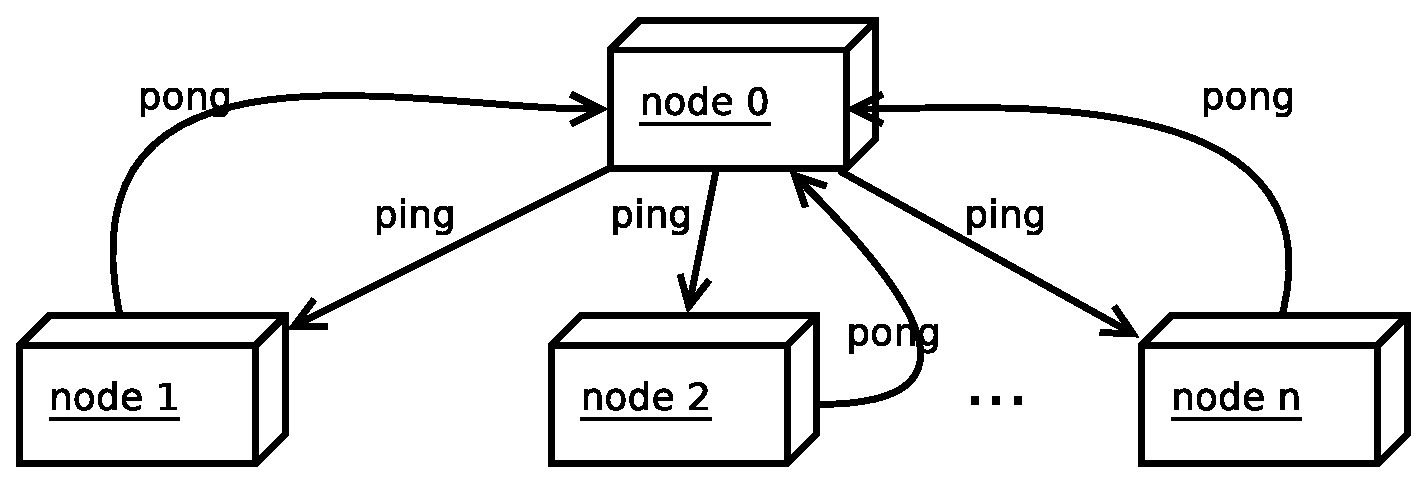
\includegraphics[width=0.5\textwidth]{node-monitoring.eps}
  \caption{Node monitoring}
  \label{pinging}
\end{figure}

\subsubsection{Reconfiguration}
Let's denote the failed node \emph{node k}.
When \emph{node 0} discovers that \emph{node k} failed it does the following things:
\begin{enumerate}
\item removes the failed node from configuration - not to try to send any data to it
\item if there is a barrier in progress - removes the node from the barrier.
If it is the last node the barrier is waiting for - the barrier is finished and its finish is propagated to other nodes.
See Fig. \ref{barrier} \nameref{barrier}.
\item the communication tree is updated. If, in the communication tree, \emph{node k} has two children: \emph{node i} and \emph{node j},
  they are reattached to another node that is still active. This is realized in a following manner: first, \emph{node 0} finds a leaf in a communication tree.
  Then \emph{node i} and \emph{node j} are attached to the leaf as its children. Please see Fig. \ref{communication-fix} \nameref{communication-fix}
  Note that after this operation the tree is no longer fully balanced.
\end{enumerate}



\begin{figure}
  \centering
      \includegraphics[width=0.7\textwidth]{barrier.eps}
  \caption{Continuing barrier after node failure}
  \label{barrier}
\end{figure}

\begin{figure}
  \centering
      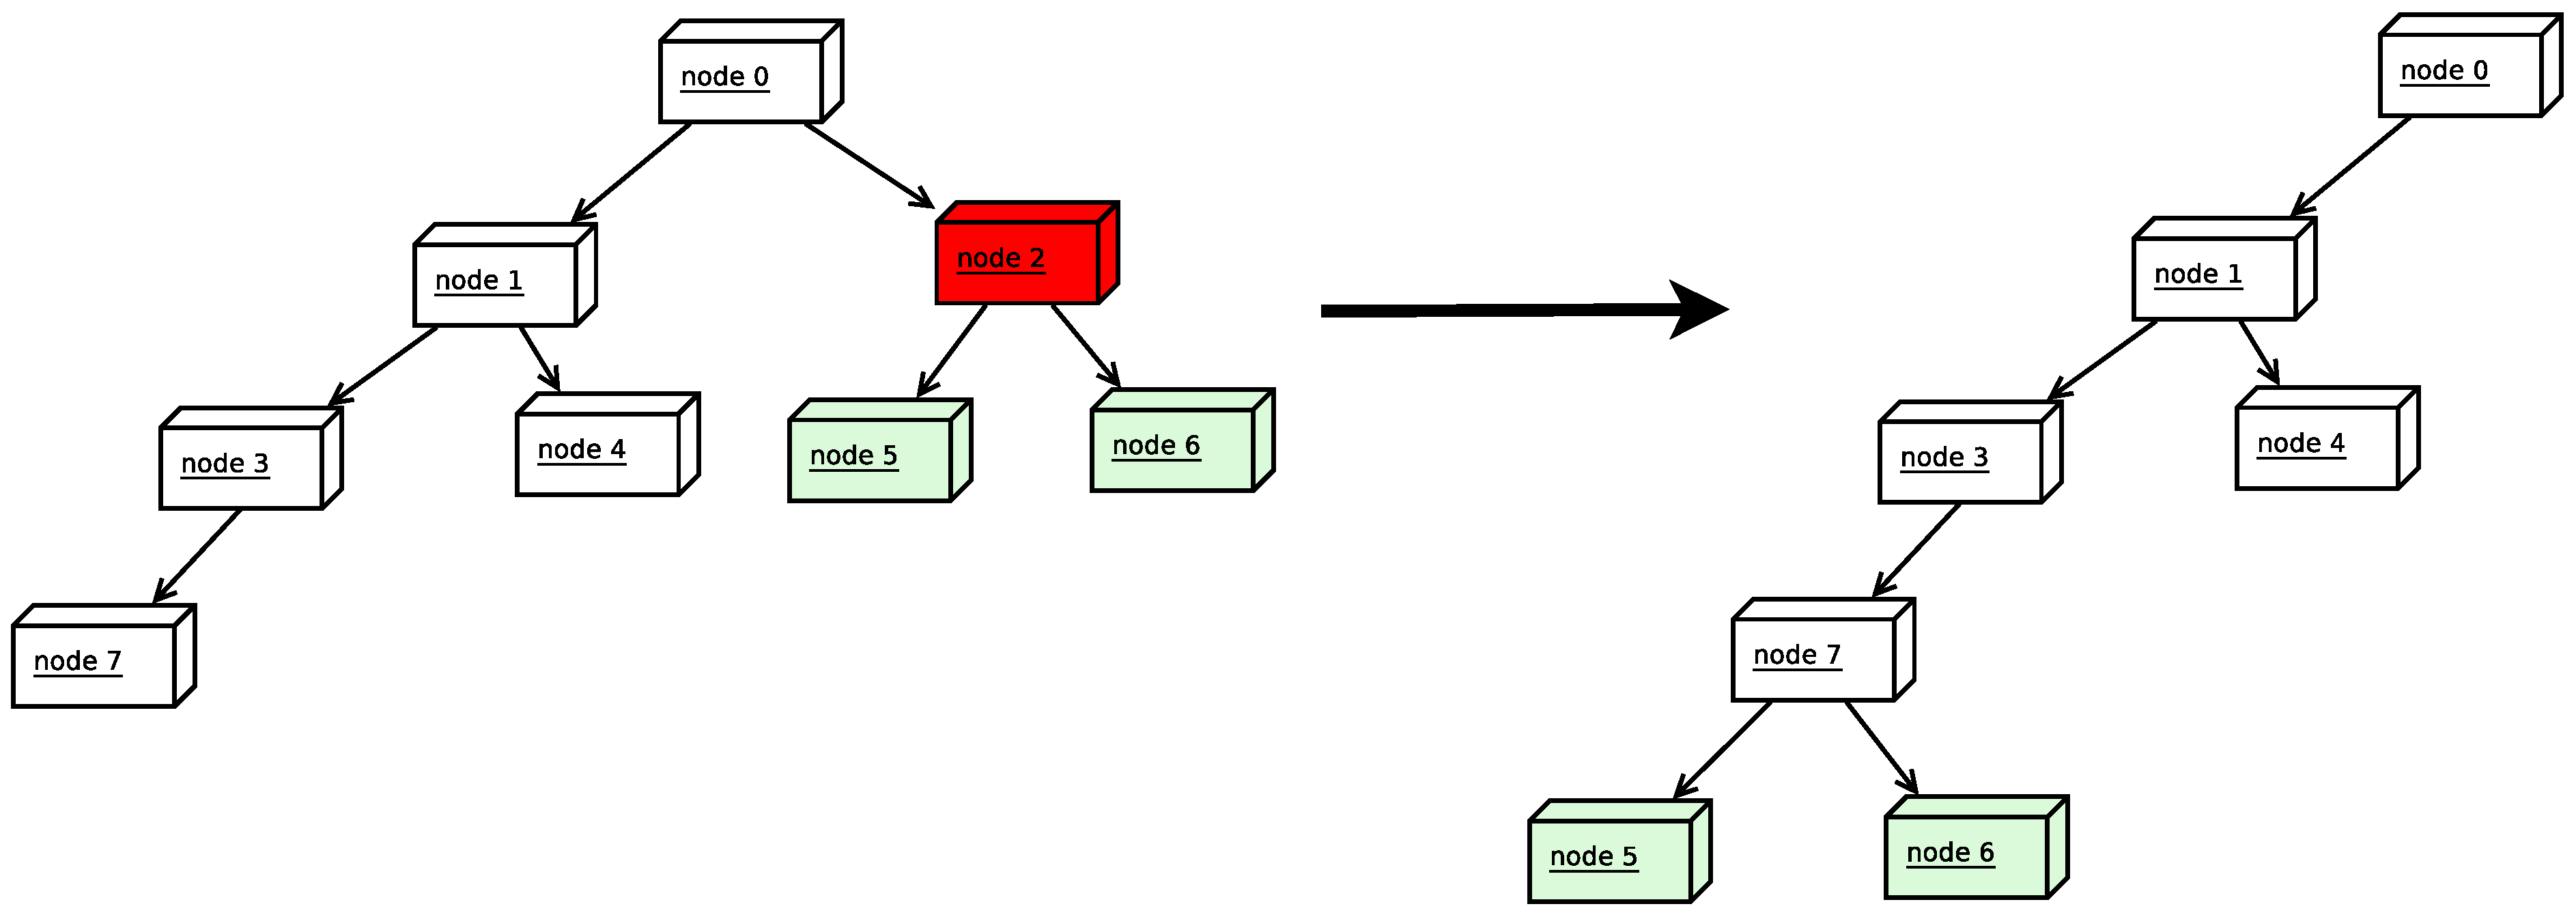
\includegraphics[width=1\textwidth]{communicatio-tree-fix.eps}
  \caption{Fixing communication tree}
  \label{communication-fix}
\end{figure}

\subsubsection{Replaying communication}
Node failure can cause loss of underlying communication.

Let's take a look at \inlinecode{barrier}.
As described in \ref{sync}, when barrier is reached by all threads, \emph{node 0} broadcasts a message that releases the barrier to all nodes.
When \emph{node k} fails during broadcast and it has \emph{node i} and \emph{node j} as children, \emph{node i} and \emph{node j} will not get this message and hang.

To prevent this situation \emph{node l}, which is established a new communication parent for \emph{node i} and \emph{node j}, has to replay communication.
Since a node can never know in advance when it will become a communication parent, every node stores all broadcast communication that it gets to be able to resend.
Messages are stored for some amount of time and evicted when the time passes.

When \emph{node i} and \emph{node j} are attached to \emph{node l}, \emph{node l} sends all broadcast messages to \emph{node i} and \emph{node j}.
It might happen that a message was already processed on e.g. \emph{node i}.
Each message is given a unique identifier. Based on this identifier, PCJ internals figure out if the message has been already processed or not.
If it has not, the message is processed and sent further in the communication tree. If it has, the message is only passed through.

\subsection{Performance overhead}
To check performance overhead of introduced changes, a test that invoked barriers one by one was executed.
The test was performed on a 4 core machine with 20 PCJ nodes.

Fig. \ref{performance} \nameref{performance} shows results of the test.
Each result is a median of three test runs.

TODO: analyze



\begin{figure}
  \centering
      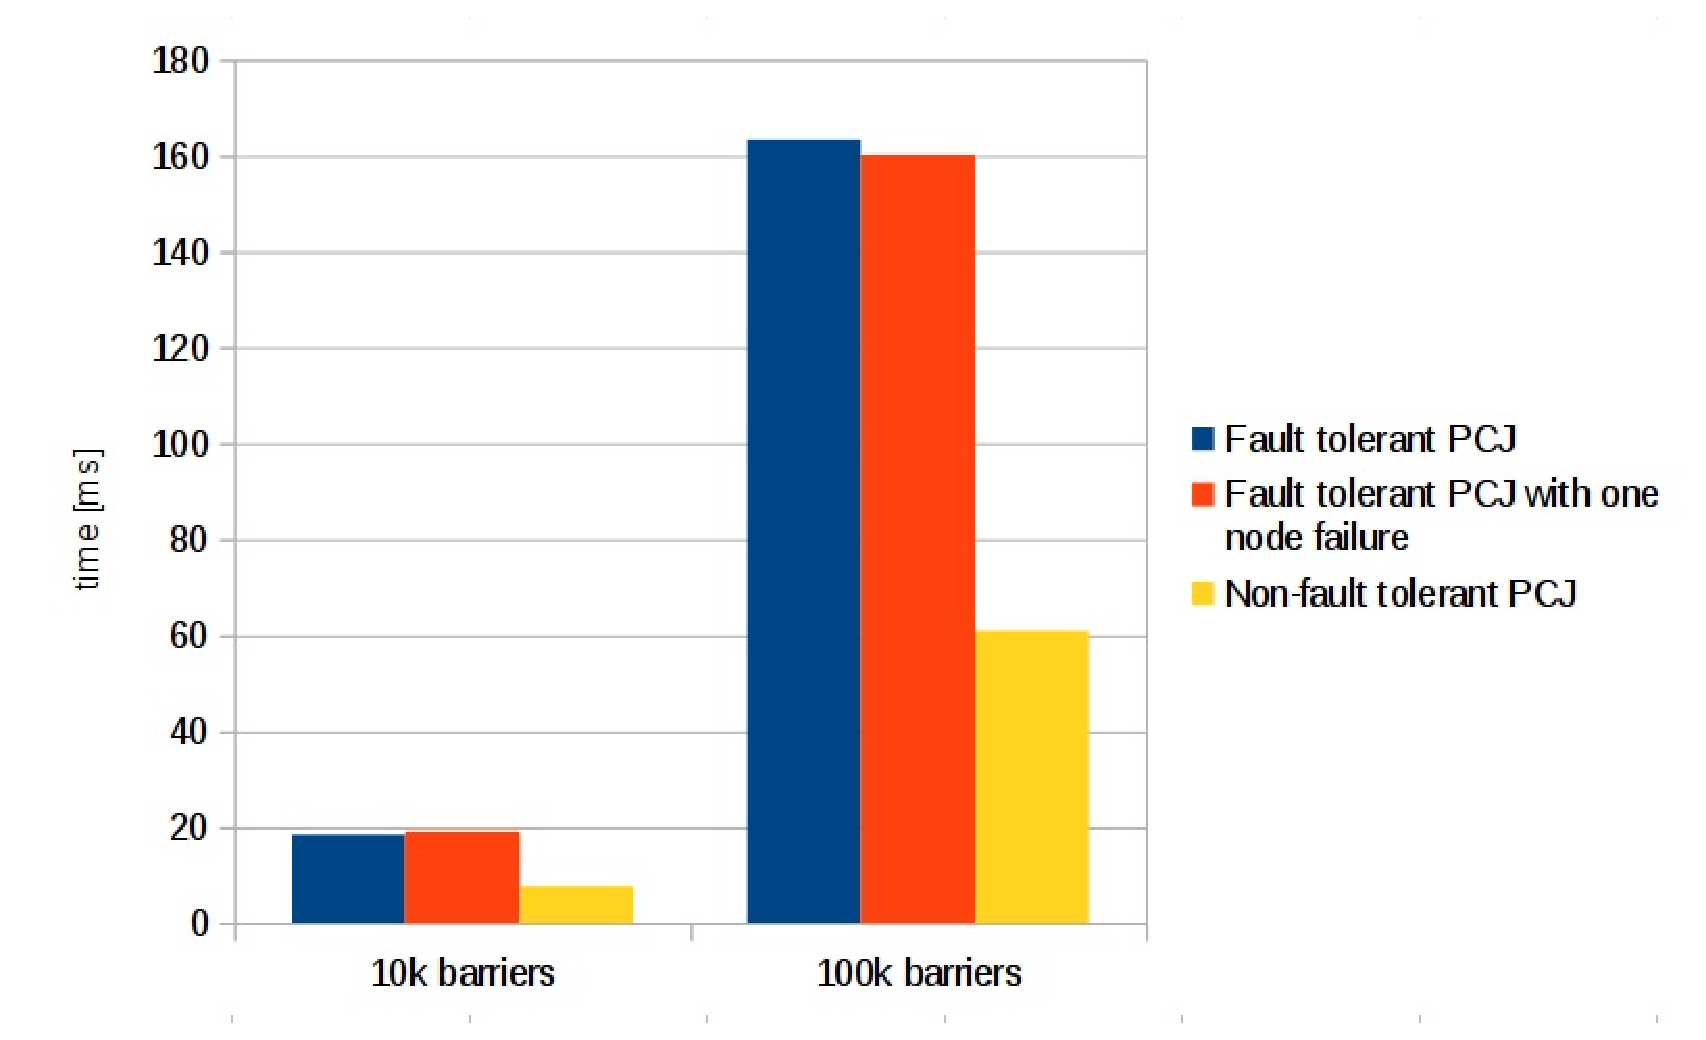
\includegraphics[width=1\textwidth]{barrier-test-chart.eps}
  \caption{Performance comparison}
  \label{performance}
\end{figure}


\section{Future work}

%Moreover we plan to provide a resilient storage to make it possible to restore thread state from a snapshot.
%Resilient storage will have two modes: synchronous and asynchronous.
%Synchronous mode will allow programs to recover from the latest position achieved by the failed thread.
%In asynchronous mode state will be saved in a storage in a non-blocking fashion.
%\\
%                \\
%%                mstodo: move descriptions elsewhere
%\section{Example use cases of strategies}
%Following are examples of possible usages of fault tolerance strategies described in this paper.
%\subsection{Ignore failure}
%The failed node is ignored, all of its data is lost.
%Might be used for instance for monte carlo randomized algorithms, e.g. monte carlo Pi approxmiation.
%\subsection{Respawn node with synchronous resilient storage}
%The most powerful strategy. Upon failure of physical node all the threads running on it are recreated on other nodes.
%Then the state of threads is recreated from the latest saved state.
%Might be used for example for parallel FFT implementation.
%In FFT implementation, in multiple phases, each thread first makes computations and then broadcasts the results.
%It is crucial to remember the exact state from the broadcasting phase.
%% mstodo: verify
%\subsection{Respawn node with asynchronous resilient storage}
%As in previous strategy, threads are recreated on active nodes.
%The state is restored from resilient storage, but since the storage is asynchronous, it might contain old data.

\subsection{Resilient storage implementation}

\section{Conclusion}

\begin{thebibliography}{1}

\bibitem{RX10}
Leslie Lamport, Dave Cunningham, Dave Grove, Ben Herta, Arun Iyengar, Kiyokuni Kawachiya, Hiroki Murata, Vijay Saraswat, Mikio Takeuchi, Olivier Tardieu
\emph{Resilient X10. Efficient failure-aware programming},
Proceedings of the 19th ACM SIGPLAN symposium on Principles and practice of parallel programming

\bibitem{pcj}
Marek Nowicki, Piotr Bała
\emph{PCJ - New Approach for Parallel Computations in Java}
Applied Parallel and Scientific Computing, 11th International Conference, PARA 2012, Helsinki, Finland, June 10-13, 2012, Revised Selected Papers
% mstodo how to cite it properly?

\bibitem{pcj-manual}
Marek Nowicki, Piotr Bała
\emph{PCJ. Parallel Computing in Java}, 2013, [Online]. Available: \url{http://pcj.icm.edu.pl/c/document_library/get_file?uuid=e8b5a416-644d-43d0-a19c-74e14555ef96&groupId=43801} [2015, April 14]

\bibitem{shmem}
Pengfei Hao, Pavel Shamis, Manjunath Gorentla Venkata, Swaroop Pophale, Aaron Welch, Stephen Poole, Barbara Chapman, \emph{Fault Tolerance for OpenSHMEM}, PGAS/OUG14
Available: \url{http://nic.uoregon.edu/pgas14/oug_submissions/oug2014_submission_12.pdf} [2015, April 17.]

\end{thebibliography}

\end{document}
